\documentclass[a4paper,11pt,twoside]{article}
\usepackage[T1]{fontenc}
\usepackage[utf8]{inputenc}
\usepackage[swedish]{babel}

\usepackage[margin=1in]{geometry}
\usepackage{amsfonts, amsmath, amssymb}
\usepackage[none]{hyphenat}
\usepackage{mathtools}

\usepackage{graphicx}

\usepackage{url}
%%  Defines the command \url{} that can be used to typeset url:s
%%  in text

\usepackage[parfill]{parskip}
\usepackage{ragged2e}

\setcounter{tocdepth}{4}
\setcounter{secnumdepth}{4}


\newcommand*{\pd}[2]{\ensuremath{\dfrac{\partial #1}{\partial #2}}}
\newcommand*{\inpd}[2]{\ensuremath{\frac{\partial #1}{\partial #2}}}
\DeclarePairedDelimiter\floor{\lfloor}{\rfloor}



\title{Matematik och Konvolutionella Neurala Nätverk för dataseende}
\title{eller}
\title{Objektdetektering och Ansiktsigenkänning med Konvolutionella Neurala Nätverk}
\title{eller}
\title{Konvolutionella neurala nätverk för ansiktsigenkänning och sifferavläsning}
\date{}


\begin{document}

\maketitle
\vfill

\begin{flushright}
\today \\*
Nikita Zozoulenko Na15b \\*
nikita.zozoulenko@gmail.com \\*
Katedralskolan i Linköping\\*
Handledare: Rickard Engström \\*
VT 2017 - HT 2018 \\*
\end{flushright}
\newpage

%start abstract
\Large{\textbf{Abstract}}\\\\
Convolutional Neural Networks are a biologically inspired machine learning model that was popularized 2012 when it won the annual ImageNet Large-Scale Visual Recognition Challenge, beating all current machine learning models. Today they have achieved state of the art results in areas such as self-driving cars, image classification, object localization, automatic image annotation, semantic segmentation and natural language processing. In this paper the mathematical model behind the standard Artificial Neural Network and the Convolutional Neural Network is derived. A Convolutional Neural Network is then adapted to read handwritten digits and to make a cutting edge face detector, successfully detecting over 50 faces in a crowded scene.
\newpage
%end abstract

\tableofcontents

\section{Inledning}

\subsection{Bakgrund}
Artificiella neurala nätverk var först introducerade på 1940-talet och simulerades med hjälp av strömkretsar. Modellen är inspirerad från hur människans hjärna är uppbyggd av ett flertal neuroner som är kopplade till varandra. Yann LeCunn uppfanna det Konvolutionella Neurala Nätverket 1998 och det var designat till att efterlikna hur ett djurs prefrontalkortex fungerar. Trots att neurala nätverk har funnits i mer än ett halvt sekel har dem inte sett stor använding innan år 2012 då ett konvolutionellt neuralt nätverk användes för att vinna den årliga ImageNet objektklassifikationstävlingen. Under de senaste 5 åren har modellen använts för att uppnå de bästa möjliga resultaten inom bland annat självkörande bilar, objektdetektering i bilder, meningsöversättning mellan olika språk och automatiskt skapande av undertexter från ljud. \cite{cs231n}

\subsection{Syfte}
Syftet med arbetet är att härleda och redogöra för den underliggande matematiken bakom den matematiska modellen av artificiella neurala nätverk och konvolutionella neurala nätverk, samt att visa exempel på praktiska tillämpningar av modellen.

\subsection{Frågeställning}
Vad är ett konvolutionellt neuralt nätverk?
Hur härleds framåt- och bakåtpropagering i konvolutionella neurala nätverk?
Hur kan modellen tillämpas för att implementera sifferavläsning, ansiktsigenkänning och objektdetektering i bilder?


\newpage
\section{Metod}
Majoriteten av tiden gick åt till se på videoföreläsningar av kursen "CS231n: Convolutional Neural Networks for Visual Recognition" från Stanford University för att få en grundläggande bakgrund och intuition om artificiella neurala nätverk. Jag implementerade sedan ett klassiskt artificiellt neuralt nätverk i C++ och python, och ett konvolutionellt neuralt nätverk i python. De partiella derivatorna som beräknas i modellen jämfördes med en analytitisk approximation med hjälp av derivatans definition. Flera forskares bloggar användes för att i mer detalj förstå matematiken bakom nätverksoperationerna. För att fördjupa mig i konvolutionella neurala nätverk läste jag de riktiga vetenskapliga artiklarna såsom Batch Normalization (Ioffe \& Szegedy, 2015) och Focal Loss (Lin et al. 2017) för att sedan implementera dem i python. När min egen implementation blev för beräkningsineffektiv började jag använda två GPU-accelererande maskininlärningsbibliotek: PyTorch och Tensorflow. 

\newpage
\section{Resultat}


\subsection{Tensorer, indexering och notation}
Tensorer är generaliseringen av vektor- och matrisbegreppen. En tensor med ordning 1 är en vektor $x \in \mathbb{R}^N$ och är en radvektor med $N$ element. Det kan dessutom tolkas som en endimensionell array. Matriser $M$ är tensorer med ordning 2 sådana att $M \in \mathbb{R}^{R \times N}$ och kan ses som en vektor av $R$ vektorer med $N$ element eller en tvådimensionell array med $R \times N$ element. En tensor med ordning $n$ indexeras med en $n$-tupel. Exempelvis indexeras en tensor $X \in \mathbb{R}^{R \times C \times H \times W}$ med fyr-tupeln $(r,c,h,w)$ där $0 \leq r < R$, $0 \leq c < C$, $0 \leq h < H$ och $0 \leq w < W$. \cite{cs231n}

% En tensor med ordningn kan ses som en tensor med ordning1 vars element är tensorer med ordningn-1. Exempelvis är en vektor en vektor av skalärer och en matris en vektor av vektorer. Funktionen $vec()$ gör om en tensor med ordningn till en vektor genom att rekursivt använda den sistnämnda egenskapen av tensorer. \cite{convmath}

\subsection{Feed-forward neurala nätverk}
Ett artificellt neuralt nätverk består av ett antal lager neuroner. De är uppbyggda rekursivt så att resultatet av ett lager är inmatningsdatan till nästintilliggande lager. Inmatningsdatan för modellen matas in i det första lagret sådant att ett neuron är ett värde. Nervsignalen propageras framåt tills den når det sista lagret. Hur nervceller från ett lager är kopplade till det föregående lagret varierar med vilket typ av neuralt nätverk man använder sig av. \cite{cs231n}

Den mest grundläggande modellen har flera namn, bland annat:  \textit{Multilayer Perceptrons} \textit{Fully Connected Cascade (FCC)}, \textit{Feed-forward Neural Network} och \textit{Densly Connected (Dense)}. Den består av ett flertal lager av neuroner. Varje neuron i ett lager är kopplade till alla neuroner i nästintillföljande lager. Nervsignalen framåtpropageras beroende på hur stark kopplingen mellan två neuroner är. Ett neurons värde kallas för dess aktivering. \cite{cs231n}

\begin{figure}[h]\label{figFCC}
	\centering
  		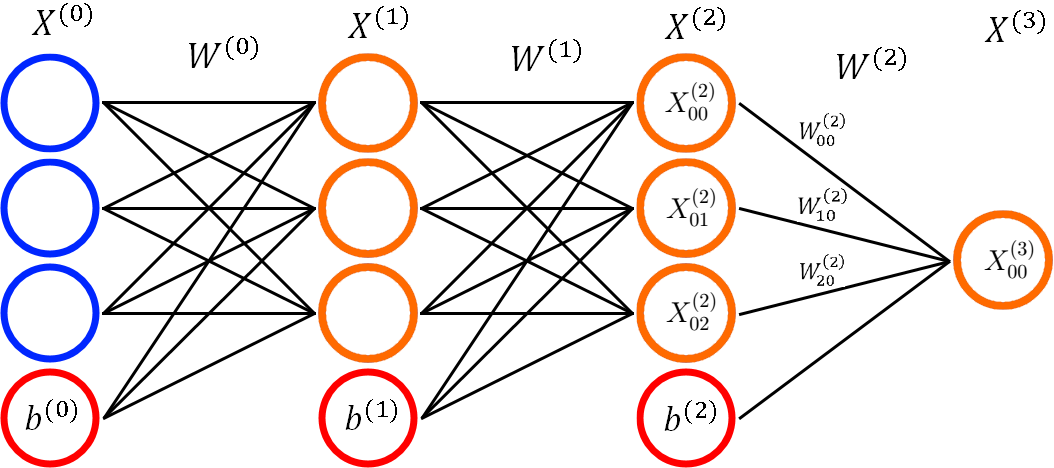
\includegraphics[scale=0.4]{FCC.png}
  	\caption{Ett exempel på ett enkelt feed-forward neuralt nätverk. Inputneuronerna är blåmarkerade medan resterande neuroner är orangea. Röda neuroner är så kallade \textit{bias-neuroner} som är konstanta oberoende på inmatningsdatan. Svarta linjer symboliserar vikterna och styrkan mellan två neuroner.}
\end{figure}

\subsubsection{Framåtprogagering}
\textit{Forward propagation} eller framåtpropagation är processen att från sina inputneuroner propagera nervsignalen framåt i nätverket tills man når det sista lagret. \cite{cs231n} \cite{wikiStanford}

Nätverket kan framställas genom att representera neuronerna och deras kopplingar med hjälp av matriser. Flera träningsexempel bearbetas samtidigt i en så kallad mini-hop med storlek R. Låt $X_{ri}^{(l)}$ benämna neuron nummer $i$ i lager $l$ i träningsexempel $r$. $W_{ba}^{(l)}$ blir vikten eller styrkan på kopplingen mellan neuron $X_{ra}^{(l)}$ och $X_{rb}^{(l+1)}$. Låt $b^{(l)}$ vara ett konstant neuron kallat \textit{bias} som är kopplad till alla neuron i lager $l+1$.  \cite{cs231n} \cite{wikiStanford}

Värdet för ett godtyckligt neuron kallas för den neuronens aktivering. För att beräkna aktiveringen av ett neuron i lager $l+1$ multipliceras varje neurons värde i lager $l$ med deras korresponderande vikt i viktmatrisen $W^{(l)}$. Resultaten och lagrets konstanta neuron $b^{(l)}$ summeras och summan matas in i en aktiveringsfunktion $f(x)$. Funktionsvärdet blir aktiveringen för det nya neuronet i lager $l+1$. Exempelvis kan signalöverföringen mellan lager 2 och 3 för ett godtyckligt exempel $r$ i mini-hopen i figur 1 beskrivas matematiskt genom: \cite{cs231n} \cite{wikiStanford}

\begin{align}
Z_{r0}^{(3)} & = X_{r0}^{(2)}W_{r0}^{(2)} + X_{r1}^{(2)}W_{10}^{(2)} + X_{r2}^{(2)}W_{20}^{(2)} + b^{(2)} \\
X_{r0}^{(3)} & = f(Z_{r0}^{(3)})
\end{align}
%& = f(X^{(2)}W^{(2)} +b^{(2)})

Där $X^{(3)} \in \mathbb{R}^{1 \times 1}$, $X^{(2)} \in \mathbb{R}^{1 \times 3}$, $W^{(2)} \in \mathbb{R}^{3 \times 1}$ och $b^{(2)} \in \mathbb{R}^{1}$.

Neuronmatriserna och viktmatriserna är definierade på ett sådant sätt att framåtpropegationen mellan lager $l$ och $l+1$ kan beräknas med en matrismultiplikation och kan därför beräknas rekursivt från inputneuronerna: \cite{cs231n} \cite{wikiStanford}
\begin{align}\label{feed-forward}
Z_{r,i}^{(l+1)} & = [X^{(l)}W^{(l)}]_{r,i}+b^{l}\\
X_{r,i}^{(l+1)} & = f(Z_{ri}^{(l+1)})
\end{align}
Vanliga aktiveringsfunktioner för neurala nätverk är \textit{Rectified Linear Units ($ReLU$)}, \textit{sigmoid ($\sigma$)} och \textit{tangens hyperbolicus ($tanh$)}. Funktionerna måste vara deriverbara för att nätverket ska kunna tränas genom processen som kallas för bakåtpropagering. Genom att använda olinjära funktioner kan nätverket lära sig olinjära samband. Definitionerna av funktionerna ges av: \cite{cs231n} 
\begin{figure}[h]\label{aktiveringsfunktion}
	\centering
  		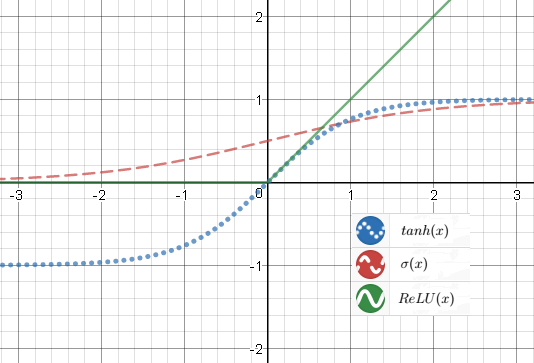
\includegraphics[scale=0.83]{activationfunction.png}
  	\caption{Grafen av aktiveringsfunktionerna $ReLU$, $\sigma$ och $tanh$.}
\end{figure}

\begin{equation}
ReLU(x) = \begin{cases} 
			0 & \mbox{om } x < 0 \\ 
			x & \mbox{om } x \geq 0 
		\end{cases}
\end{equation}

\begin{equation}
\sigma(x) = \frac{1}{1+e^{-x}}
\end{equation}

\begin{equation}
tanh(x) = \frac{e^x-e^{-x}}{e^x+e^{-x}}
\end{equation}

\subsubsection{Kostnadsfunktionen}
Givet ett inmatningsvärde $X$ skapas ett närmevärde $\hat{y}$ som ska vara så nära det sanna värdet för y som möjligt. Initialt kommer $W^{(l)}$ vara slumpade för varje lager $l$ och nätverkets prognos kommer inte efterlikna det sökta värdet. Med hjälp av \textit{gradient descent} kan man iterativt träna modellen så det slutgiltiga värdet kommer så nära $y$ som möjligt. Detta görs genom att definiera en multivariat kostnadsfunktion $L(W, b; X,y)$ av alla nätverkets parametrar med avseende på ett träningsexempel $(X, y)$. Funktionen är ett mått på prognosen $\hat{y}$ kvalitet. Man definierar $L$ på ett sådant sätt att ju mindre värdemängd av $L$, desto högre kvalitet består $\hat{y}$ av. Ett sätt att definiera $L$ är exempelvis med en så kallad \textit{L2 kostnadsfunktion}: \cite{cs231n} \cite{wikiStanford}
\begin{equation}
\begin{split}
L(\theta) 	& = {||\hat{y}-y||}^2 \\
		& = {||f(f(f(XW^{(0)} +b^{(0)})W^{(1)} +b^{(1)})W^{(2)} +b^{(2)}) - y||}^2
\end{split}
\end{equation}
Träningen av det neurala nätverket är processen där man hittar konstnadsfunktionens minimum med hjälp av \textit{gradient descent}.

\subsubsection{Gradient Descent}
Gradienten $\nabla L(\theta)$ är en vektor av partiella derivator med avseende på funktionen $L$ variabler $W^{(0)}$, $W^{(1)}$, ..., $W^{(l)}$, $b^{(0)}$, $b^{(1)}$, ..., $b^{(l)}$ som definieras genom: \cite{gradient} \cite{convmath} 
\begin{equation}
\nabla L(\theta) : \mathbb{R}^n \to \mathbb{R}^n
\end{equation}
\begin{equation}
\nabla L(\theta) = 
	\begin{pmatrix} 
		\pd{L(\theta)}{\theta^{(0)}} & 
		\pd{L(\theta)}{\theta^{(1)}} &
		\cdots &
		\pd{L(\theta)}{\theta^{(n-1)}}
		
		\end{pmatrix}
\end{equation}

Gradienten $\nabla L(\theta)$ visar riktningen vari värdemängdsökningen är som störst. Genom att ändra vikterna $\theta$ värde proportionellt med avseende på den negativa gradienten $-\nabla L(\theta)$ kan man iterativt modifiera $\theta$ tills man når funktionens minimum. Den mest grundläggande algoritmen för \textit{gradient descent} kallas för \textit{Stochastic Gradiant Descent (SGD)} och använder hyperparametern $\alpha$ för att beteckna träningshastigheten: \cite{gradient} \cite{convmath} \cite{wikiStanford}

\begin{equation}
\pd{L(\theta)}{\theta^{(l)}} = \nabla_{\theta^{(l)}} L(\theta)
\end{equation}
\begin{equation}\label{SGD}
\theta^{(l)} \to \theta^{(l)} - \alpha \pd{L(\theta)}{\theta^{(l)}}
\end{equation}
\begin{figure}[h]\label{figSGD}
	\centering
  		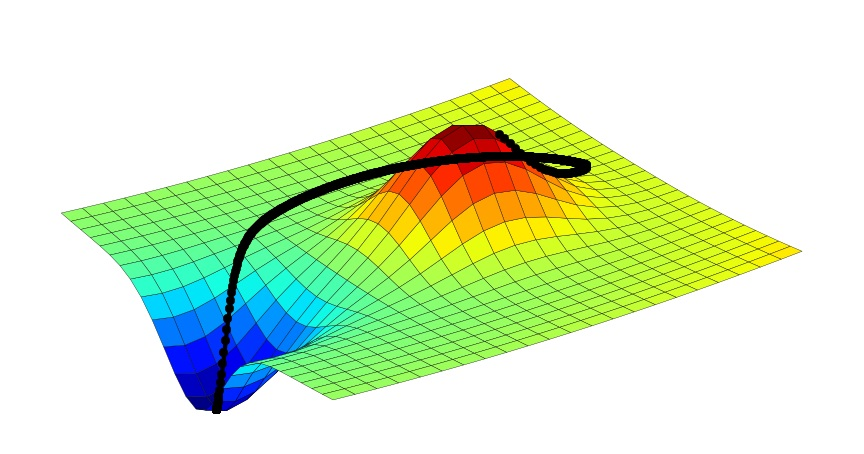
\includegraphics[scale=0.5]{SGD.png}
  	\caption{En illustration av gradient descent på en funktion med två variabler.\cite{figSGD}}
\end{figure}
Nätverket tränas genom att varje träningsexempel $(X,y)$ framåtpropageras och insätts i kostnadsfunktionen $L$. Genom processen som kallas för bakåtpropagering beräknas alla partiella derivator med avseende på en viss vikt och används för att uppdatera vikterna tills nätverkets prognos liknar de sanna värdena. \cite{gradient} \cite{convmath} \cite{wikiStanford}
\subsubsection{Bakåtpropagering}
De partiella derivatorna kan approximeras med hjälp av framåt, bakåt eller central differenskvot för partiella derivator: \cite{wikiStanford} \cite{gradient}

\begin{equation}
\pd{L(\theta)}{\theta^{(i)}} = \frac{L(\theta^{(0)},...,\theta^{(i)} + h, ..., \theta^{(n-1)})-L(\theta)}{h}
\end{equation}

Detta skulle inte skapa några problem för det lilla neurala nätverket i figur 1 med 24 parametrar, men i själva verket har djupa neurala nätverk miljontals av parametrar som behöver en enorm datorkraft. Istället tillämpas regler för differentialkalkyl för att effektivt beräkna de partiella derivatorna. För ett godtyckligt lager $l$ används kedjeregeln för att bryta upp derivatan av $L$ med avseende på en vikt i tre bråk. På grund av att alla träningsexempel i mini-hopen använder vikten i fråga summeras alla exempel i mini-hopen $R$. För derivatan av de konstanta neuronerna summeras alla partiella derivator för det lagret. För att sambandet mellan två neuroner och en godtycklig vikt är linjär kan det enkelt deriveras. \cite{cs231n}

Låt
\begin{equation}
\inpd{L(\theta)}{X^{(l)}} = \delta^{(l)}
\end{equation}
Derivatan av $L$ med avseende på ett lagers parameter beräknas genom: \cite{cs231n}
\begin{equation}\label{dLdW_FCC}
\begin{split}
\pd{L(\theta)}{W^{(l)}_{j,i}} 
	& = \sum^{R-1}_{r=0} \pd{L(\theta)}{X^{(l+1)}_{r,i}} \pd{X^{(l+1)}_{r,i}}{Z^{(l+1)}_{r,i}} \pd{Z^{(l+1)}_{r,i}}{W^{(l)}_{i,j}} \\
	& = \sum^{R-1}_{r=0} \delta^{(l+1)}_{r,i} f'(Z^{(l+1)}_{r,i}) \ X^{(l)}_{r,j}\\
\end{split}
\end{equation}
\begin{equation}\label{dLdb_FCC}
\begin{split}
\pd{L(\theta)}{b^{(l)}} 
	& = \sum^{R-1}_{r=0} \pd{L(\theta)}{X^{(l+1)}_{r,i}} \pd{X^{(l+1)}_{r,i}}{Z^{(l+1)}_{r,i}} \pd{Z^{(l+1)}_{r,i}}{b^{(l)}_{i,j}} \\
	& = \sum^{R-1}_{r=0} \delta^{(l+1)}_{r,i} f'(Z^{(l+1)}_{r,i}) \\
\end{split}
\end{equation}
$\delta^{(l)}$, också kallat \textit{delta-felet}, är enligt dess definition derivatan av $L$ med avseende på ett visst neuron. Det kan tolkas som hur känslig värdemängdsförändringen för kostnadsfunktionen är för ett visst neuron vid lager $l$. En vikt kopplat till ett neuron med högt delta-fel är mer ansvarig för skiftning i kostnaden än ett neuron med lågt delta-fel. Genom att propagera nervsignalen baklänges i nätverket med kostnadsfunktionens värde som inputvärde kan man beräkna alla neuroner $X^{(l)}$ påverkan på $L$ vid ett godtyckligt lager $l$. \cite{cs231n}

Bakåtpropageringen av delta-felen uttrycks rekursivt från det sista lagret $\hat{y}$. Delta-felet vid det sista lagret $l_{sista}$ beror på kostnadsfunktionen. För en L2 kostnadsfunktion definieras delta-felet som: \cite{cs231n}
\begin{equation}
\begin{split}
\delta^{(l_{sista})}
	& = \pd{L(\theta)}{\hat{y}}  \\
	& = 2 ||\hat{y}-y||
\end{split}
\end{equation}
Likt ekvation \eqref{dLdW_FCC} summeras alla  partiella derivator av neuronerna vid användingen av kedjeregeln: \cite{cs231n}

\begin{equation}\label{dLdX_FCC}
\begin{split}
\delta^{(l)}_{r,i}
	& = \pd{L(\theta)}{X^{(l)}_{r,i}}  \\
	& = \sum^{N'}_{j=0} \pd{L(\theta)}{X^{(l+1)}_{r,j}} \pd{X^{(l+1)}_{r,j}}{Z^{(l+1)}_{r,j}} \pd{Z^{(l+1)}_{r,j}}{X^{(l)}_{r,i}} \\
	& = \sum^{N'}_{j=0} \delta^{(l+1)}_{r,j} f'(Z^{(l+1)}_{r,i}) \ W^{(l)}_{j,i} 
\end{split}
\end{equation}

Bakåtpropageringen sker lager till lager med start i outputlagret. Vid varje lager måste delta-felet $\delta^{(l)}$ bakåtpropageras och derivatan av det lagrets parametrar $W^{(l)}$ och $b^{(l)}$ beräknas. \cite{cs231n}

\subsection{Träning av neurala nätverk}
Neurala nätverk tränas genom att iterativt uppdatera nätverkets vikter med hjälp av \textit{gradient descent}. Den hela träningsdatabasen delas in i mini-hopar och väljs ut slumpvist. En iteration av SGD appliceras genom att framåtpropagera ett träningsexempel och sedan bakåtpropagera felet för att beräkna gradienten av kostnadsfunktionen med avseende på alla vikter i närverket. Denna process upprepas tills nätverkets vikter konvergerar och nätverkets prognos efterliknar verkligheten. \cite{cs231n}

Två implementationer av ett feed-forward neuralt nätverk kan hittas på github i python och C++: \url{https://github.com/nikitazozoulenko}

\subsection{Konvolutionella neuala nätverk}
När människor vill identifiera någonting i en bild så letar vi efter vissa karakteristiska drag objektet har. En hund består exempelvis av en kropp, ett huvud och fyra ben. Kroppsdelarna består sedan själva av grundläggande geometriska former som i sig självt är kombinationer av kanter och linjer. Dessutom har hundar en viss textur, det som vi kännetecknar som något pälsliknande. Dessa karakteristiska drag är lokala inom bilden och kan extraheras av att endast se på en liten del av bilden i taget. Detta är principen bakom \textit{Konvolutionella Neurala Nätverk (CNN)}: Genom så kallade \textit{konvolutioner} kunna extrahera dessa karakteristiska drag. Nätverket lär sig ett antal små filter som den applicerar på en delmängd av bilden genom att filtret sammanrullar över hela bilden (se figur 4). Värdet av filtret över en delmängd av bilden blir aktiveringen av ett neuron i nästa lager. \cite{cs231n}

\begin{figure}[h]\label{figkatter}
	\centering
  		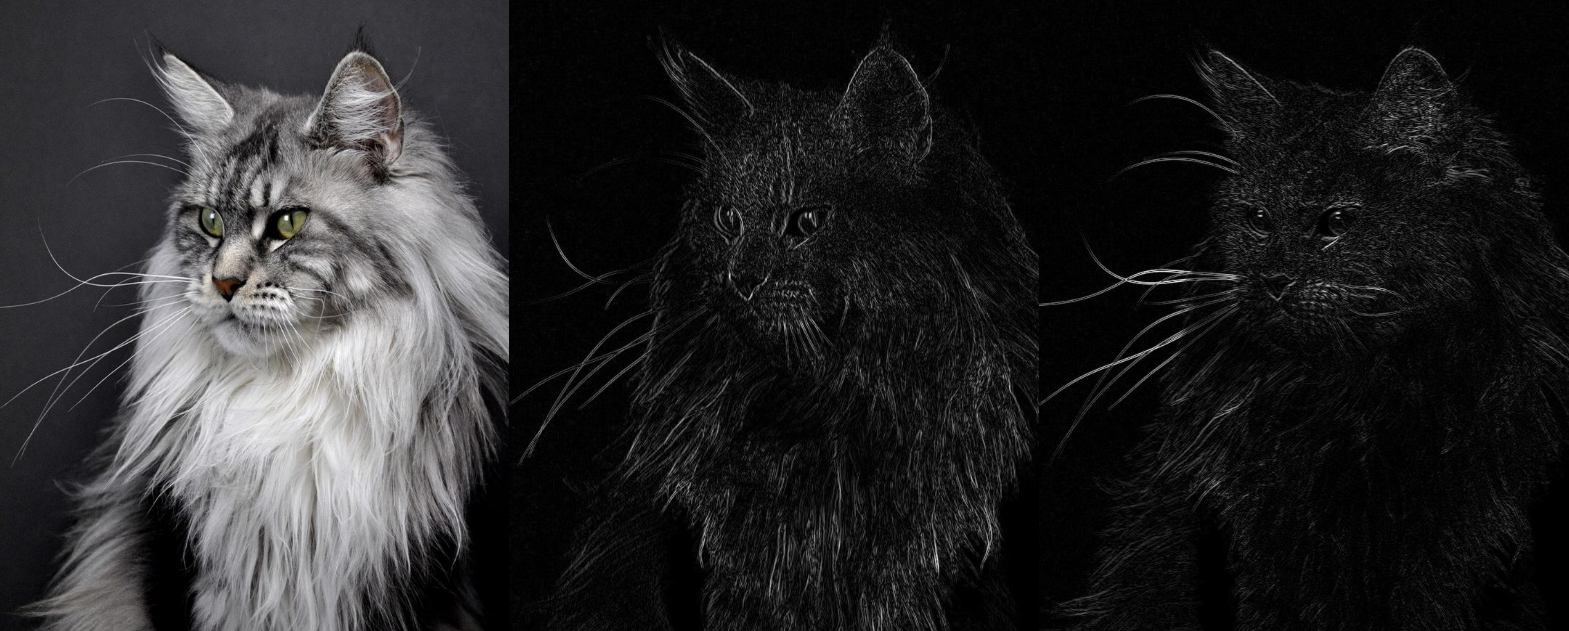
\includegraphics[scale=0.33]{katter.png}
  	\caption{Resultatet av att ett filter för vertikal respektive horizontell kantdetektering har sammanrullat över en bild av en katt.}
\end{figure}

Till skillnad från \textit{FCC} är neuronerna i ett \textit{CNN} bara kopplade till närliggande neuroner i det föregående lagret. På detta sätt kan nätverket lära sig fler hög-nivåspecialartiklar ju djupare i nätverket signalen går. Exempelvis kan det hända att det första lagret lär sig att identifiera kanter och linjer medan de senare lagren lagren lär sig att känna igen olika geometriska former och till sist känna igen ansikten eller object i det sista lagret. \cite{cs231n}

Modellen, precis som ett \textit{feed-forward nätverket}, består av ett flertal lager neuroner sådant att resultatet av ett lager matas in till nästkommande lager. Det sista lagret benämns med $X^{(l_{sista})}$ eller $\hat{y}$. Vid varje lager finns dessutom vikter $W^{(l)}$  som beror på vad för slags lager det är. $W^{(l)}$ kan vara tom med inga vikter när lager inte bidrar till någon inlärning. Ekvation \eqref{CNNeq} illustrerar strukturen av modellen.\cite{cs231n} \cite{convmath}
\begin{equation}\label{CNNeq}
X^{(0)} \xrightarrow{W^{(l)}} X^{(1)}  \xrightarrow{W^{(l)}} \cdots  \xrightarrow{W^{(l_{sista}-2)}} X^{(l_{sista}-1)}  \xrightarrow{W^{(l_{sista}-1)}} X^{(l_{sista})} = \hat{y}
\end{equation}

Samtliga olika typer av lager i en konvolutionellt neuralt nätverk har två olika faser: framåtpropagering och bakåtpropagering. Vid framåtpropagering används aktiveringen av det föregående lagret för att beräkna aktiveringen vid nästintilliggande lager. Vid bakåtpropagering måste det rekursiva delta-felet propageras baklänges i nätverket med hjälp av kedjeregeln för att sedan beräkna den paritella derivatan av lagrets vikter med avseende på kostnadsfunktionen. \cite{cs231n}

För ett feed-forward neuralt nätverk används matriser för att representera neuronerna. I ett \textit{CNN} är en tensor $X^{(l)} \in \mathbb{R}^{R \times C  \times H \times W}$ med ordning 4 aktiveringen vid lager $l$ och indexeras med fyr-tupeln $(r,c,h,w)$ där $0 \leq r < R$, $0 \leq c < C$, $0 \leq h < H$ och $0 \leq w < W$. Aktiveringarna vid nästintilliggande lager $l+1$ betecknas med $X^{(l+1)} \in \mathbb{R}^{R \times C' \times H' \times W'}$ och indexeras med fyr-tupeln $(r,c',h',w')$ där $0 \leq r < R$, $0 \leq c' < C'$, $0 \leq h' < H'$ och $0 \leq w' < W'$. \cite{cs231n} \cite{convmath}








Aktiveringen brukar illustreras som en tredimensionell volym där $W$, $H$ och $C$ är bredden, höjden respektive djupet. En $H \times W$ skiva av volymen kallas för en \textit{feature map} eller en \textit{kanal}. Antalet kanaler betecknas med $C$. $R$ står för hopstorlek då man bearbetar R exempel i taget i en så kallad mini-hop. \cite{cs231n} \cite{convmath}

\begin{figure}[h]\label{figboatcnn}
	\centering
  		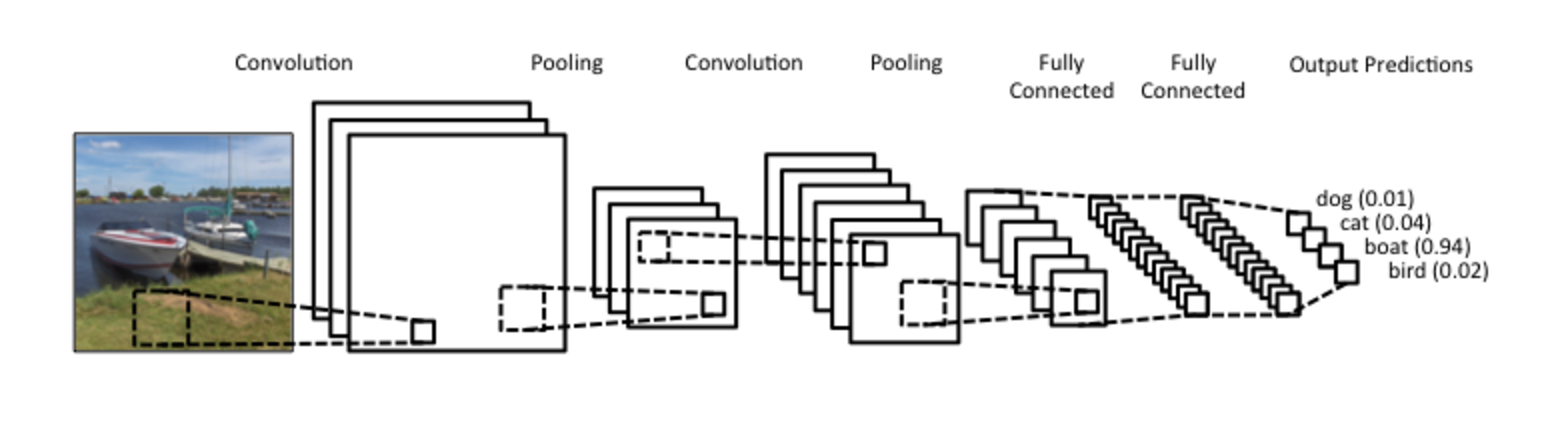
\includegraphics[scale=0.6]{boatcnn.png}
  	\caption{En illustration av ett konvolutionellt neuralt nätverk. Varje skiva är en egen \textit{feature map}. \cite{figboatcnn}}
\end{figure}

På grund av att en konvolution är en lokal operator används CNN:s för data som innehåller lokalt sammanhängande samband, exempelvis bilder eller ljud. Om det är en bild som bearbetas har det första lagrets aktivering $C = 3$ kanaler, en för varje RGB-kanal, och en bredd och höjd lika med bildens bredd och höjd i pixlar. \cite{cs231n} \cite{convmath}

\subsubsection{Konvolutionslagret framåtpropagering}
Ett konvolutionslager består av ett antal vikter kallade \textit{kärnor (kernels)} eller \textit{masker (masks)}, representerade av en tensor med ordning fyra, $W^{(l)} \in \mathbb{R}^{C' \times C  \times K_h \times K_W}$ för lager $l$. \cite{cs231n} \cite{convmath}

När masken är över en godtycklig del av volymen multipliceras varje värde i delmängden av $W^{(l)}$ elementvis med respektive värde i masken vid samma position och summeras (se figur 6). Summan blir aktiveringen av ett neuron i nästa lager. Konvolutionsoperatorn betecknas med $*$. \cite{cs231n} \cite{convmath}

\begin{figure}[h]\label{figkonv}
	\centering
  		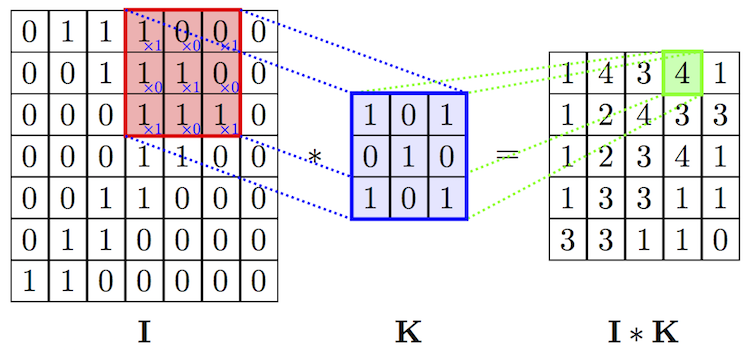
\includegraphics[scale=2.1]{convolution.png}
  	\caption{En kärna med storlek $3 \times 3$ sammanrullar över ett område med dimensioner $6 \times 6$ och bildar en aktivering med dimensionerna $4 \times 4$. \cite{figkonv}}
\end{figure}

En feature map i lager $l+1$ är resultatet av att en kärna med dimensioner $1 \times \times C  \times K_h \times K_W$ har sammanrullat över aktiveringen av det föregående lagret. $C'$ är antalet kärnor och blir dessutom antalet feature maps nästa lager har. \cite{cs231n} \cite{convmath}

Kärnorna har två ytterligare egenskaper: ett kliv $s$ och så kallad \textit{zero-padding} $p$. $s$ är hur stort kliv man tar efter varje gång filtret blir applicerat på tensorn. Man ökar tensorns höjd och bredd med $2p$ genom att fylla på med nollor vid tensors ändor (se figur 7). På grund av att aktiveringens höjd och bredd avtar ju djupare i nätverket de befinner sig på används zero-padding för att kontrollera storleken av tensorn. \cite{cs231n} \cite{convmath} \cite{convarithmetic}

\begin{figure}[h]\label{figzeropad}
	\centering
  		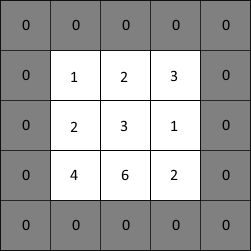
\includegraphics[scale=0.7]{zeropadding.png}
  	\caption{Ett område med dimensioner $3 \times 3$ zero-paddas med $p=1$ och resulterande område får dimensioner $5 \times 5$.}
\end{figure}

Låt $W^{(l)} \in \mathbb{R}^{C' \times C  \times K_h \times K_W}$, $X^{(l)} \in \mathbb{R}^{R \times C  \times (H+2p) \times (W+2p)}$ och $X^{(l+1)} \in \mathbb{R}^{R \times C'  \times H' \times W'}$. Dimensionerna vid lager $l+1$ beskrivs av: \cite{cs231n} \cite{convmath} \cite{convarithmetic}
\begin{equation}
W' = \frac{W-K_W+2p}{s} +1
\end{equation}
\begin{equation}
H' = \frac{H-K_H+2p}{s} +1
\end{equation}

Då beskrivs en konvolution algebraiskt genom: \cite{cs231n} \cite{convmath}
\begin{equation}
w = sw'
\end{equation}
\begin{equation}
h = sh'
\end{equation}
\begin{equation}\label{konvolution}
\begin{split}
	\begin{bmatrix} X^{(l+1)} \end{bmatrix}_{r, c', h', w'}	
		& = X^{(l)}_{r, c', h', w'} *W^{(l)}_{c'} \\
		& = \sum^{C-1}_{c=0} \sum^{K_H-1}_{j=0} \sum^{K_W-1}_{i=0} X^{(l)}_{r, c, h'+j, w'+i}W^{(l)}_{c', c, j, i}
\end{split}
\end{equation}

Index på termen som ska sammanrullas i konvolutionen symboliserar vilka dimensioner som ska summeras. Exempelvis visar $W^{(l)}_{c'}$ att dimensionerna $C$, $H$ och $W$ (alla kanaler) ska summeras medan  $W^{(l)}_{c', c}$ visar att endast $H$ och $W$ (en kanal) ska summeras.

I praktiken brukar konvolutioner implementeras med hjälp av funktionerna $row2im$ och $im2row$ vilka möjliggör att en konvolution att beräknas med en matrismultiplikation. \cite{cs231n} \cite{convmath} \cite{convarithmetic}

\subsubsection{Konvolutionslagret bakåtpropagering}
Vid varje lager $l$ bakåtpropageras det rekursiva delta-felet $\delta$ och den partiella derivatan av lagerts vikter med avseende på kostnadsfunktionen $L$ beräknas. 

Bakåtpropageringen av det rekursiva delta-felet $\inpd{L(W)}{X^{(l+1)}_{r,c',h',w'}}$ räkas ut med hjälp av kedjeregeln. Derivatan kan inte endast delas upp i $\inpd{L(W)}{X^{(l+1)}_{r,c',h',w'}}$ och $\inpd{X^{(l+1)}_{r,c',h',w'}}{X^{(l)}_{r,c,h,w}}$, utan alla derivator måste summeras på grund av att det är mer än ett neuron som är ansvarig för framåtpropageringen likt ekvationer \eqref{dLdW_FCC}, \eqref{dLdb_FCC} och \eqref{dLdX_FCC}. $X^{(l+1)}_{r,c',h',w'}$ byts sedan ut mot dess definition enligt ekvation \eqref{konvolution}. \cite{convmath} \cite{webconv1} \cite{webconv2} \cite{webconv3}
\begin{equation}\label{konvolutionbackprop}
\begin{split}
	\delta^{(l)}_{r,c,h,w}
		& = \pd{L(W)}{X^{(l)}_{r,c,h,w}} \\
		& = \sum^{C'-1}_{c'=0} \sum^{H'-1}_{h'=0} \sum^{W'-1}_{w'=0} \pd{L(W)}{X^{(l+1)}_{r,c',h',w'}} \pd{X^{(l+1)}_{r,c',h',w'}}{X^{(l)}_{r,c,h,w}} \\
		& = \sum^{C'-1}_{c'=0} \sum^{H'-1}_{h'=0} \sum^{W'-1}_{w'=0} \delta^{(l+1)}_{r,c',h',w'} \pd{\sum^{C-1}_{c=0} \sum^{k_H-1}_{j=0} \sum^{k_W-1}_{i=0} X^{(l)}_{r, c, h'+j, w'+i}W^{(l+1)}_{c', c, j, i}}{X^{(l)}_{r,c,h,w}}
\end{split}
\end{equation}

Varje produkt i den innersta summan kommer att vara lika med noll förutom om $X^{(l)}_{r, c, h'+j, w'+i} = X^{(l)}_{r,c,h,w}$. Förljaktligen insätter man $h'+j = h$ och $h'+j = h$. Summorna och derivatan förkortas: \cite{webconv1} \cite{webconv2} \cite{webconv3}
\begin{multline}
\sum^{C'-1}_{c'} \sum^{H'-1}_{h'=0} \sum^{W'-1}_{w'=0} \delta^{(l+1)}_{r,c',h',w'} \pd{\sum^{C-1}_{c=0} \sum^{K_H-1}_{j=0} \sum^{K_W-1}_{i=0} X^{(l)}_{r, c, h'+j, w'+i}W^{(l+1)}_{c', c, j, i}}{X^{(l)}_{r,c,h,w}} \\
	 = \sum^{C'-1}_{c'=0} \sum^{H'-1}_{h'=0} \sum^{W'-1}_{w'=0} \delta^{(l+1)}_{r,c',h',w'} W^{(l+1)}_{c', c, j, i} \\
	 = \sum^{C'-1}_{c'=0} \sum^{H'-1}_{h'=0} \sum^{W'-1}_{w'=0} W^{(l+1)}_{c', c, (h-h'), (w-w')}  \delta^{(l+1)}_{r,c',h',w'}   \\
\end{multline}
Vilket man kan se är en summa av konvolutioner där en viss \textit{feature map} av delta-felet sammanrullar över alla kärnor på en viss \textit{feature map} med vikter som är roterade $180^\circ$. För att en konvolution ska kunna ske måste den roterade vikten zero-paddas på grund av att det glidande fönstret måste vara som mest lika stor som tensorn den sammanrullar över. Låt rotationen betecknas med funktionen $rot()$. \cite{webconv1} \cite{webconv2} \cite{webconv3}
\begin{equation}
\delta^{(l)}_{r,c,h,w} = \sum^{C'-1}_{c'=0} rot(W^{(l+1)}_{c',c,h,w}) * \delta^{(l+1)}_{r,c'}
\end{equation}
En sundshetskontroll visar att detta är intuitivt då alla \textit{feature maps} i $X^{(l)}$ används för att skapa en enstaka \textit{feature map} i $X^{(l+1)}$. Det är därför man summerar över alla kärnor och endast konvolverar i en \textit{feature map} i taget och summerar alltihop. \cite{cs231n}

Den partiella derivatan av kostandsfunktionen med avseende på vikterna hittas på ett liknande sätt. Här summeras dessutom $R$-dimensionen på grund av att alla exempel i mini-hopen har en påverkan på gradienten: \cite{cs231n} \cite{webconv1} \cite{webconv2} \cite{webconv3} 
\begin{align}
\begin{split}
	\pd{L(W)}{W^{(l)}_{c',c,h,w}}
		& = \sum^{R-1}_{r=0} \sum^{C'-1}_{c'=0} \sum^{H'-1}_{h'=0} \sum^{W'-1}_{w'=0} \pd{L(W)}{X^{(l+1)}_{r,c',h',w'}} \pd{X^{(l+1)}_{r,c',h',w'}}{W^{(l)}_{r,c,h,w}} \\
		& = \sum^{R-1}_{r=0} \sum_{c'=0}^{C'-1} \sum^{H'-1}_{h'=0} \sum^{W'-1}_{w'=0} \delta^{(l+1)}_{r,c',h',w'} \pd{\sum\limits^{C-1}_{c=0} \sum\limits^{K_H-1}_{j=0} \sum\limits^{K_W-1}_{i=0} X^{(l)}_{r, c, h'+j, w'+i}W^{(l)}_{c', c, j, i}}{W^{(l)}_{c',c,h,w}} \\
		& = \sum^{R-1}_{r=0} \sum^{C'-1}_{c'=0} \sum^{H'-1}_{h'=0} \sum^{W'-1}_{w'=0} X^{(l)}_{r, c, h'+h, w'+w} \delta^{(l+1)}_{r,c',h',w'} \\
		& = \sum^{R-1}_{r=0} \sum^{C'-1}_{c'=0} X^{(l)}_{r, c, h, w} * \delta^{(l+1)}_{r,c'} \\
\end{split}
\end{align}

\subsubsection{Aktiveringsfunktionslager framåtpropagering}
Aktiveringsfunktionen $f$ appliceras elementvis på alla neuroner i $X^{(l)}$. Följaktligen har $X^{(l)}$ och $X^{(l+1)}$ samma dimensioner. Låt aktiveringsfunktionen betecknas med $f$. Nervsignalen framåtpropageras genom: \cite{convmath}
\begin{equation}
X^{(l+1)}_{r,c,h,w} = f(X^{(l)}_{r,c,h,w})
\end{equation}
Aktiveringsfunktioner ökar nätverks precision och får dem att konvergera snabbare, vilket leder till att mindre datakraft krävs för att träna nätverket. \cite{cs231n}

\subsubsection{Aktiveringsfunktionslager bakåtpropagering}
Aktiveringsfunktioner har inga parametrar som ska optimeras och sålades är $W^{(l)}$ och $\inpd{L(W)}{W^{(l)}}$ tomma. Bakåtpropageringen av det rekursiva delta-felet härleds med hjälp av kedjeregeln: \cite{cs231n} \cite{convmath}

\begin{equation}
\begin{split}
\delta^{(l)}_{r,c,h,w}
		& = \pd{L(W)}{X^{(l)}_{r,c,h,w}} \\
		& = \pd{L(W)}{X^{(l+1)}_{r,c,h,w}} \pd{X^{(l+1)}_{r,c,h,w}}{X^{(l)}_{r,c,h,w}} \\
		& = \delta^{(l+1)}_{r,c,h,w} f'(X^{(l)}_{r,c,h,w})
\end{split}
\end{equation}

\subsubsection{Maxpoollagret framåtpropagation}
Här är igen inputneuronerna representerade av $X^{(l)} \in \mathbb{R}^{R \times C \times H \times W}$ och skapar output $X^{(l+1)} \in \mathbb{R}^{R \times C' \times H' \times W'}$. Lagret saknar vikter men har däremot hyperparametrarna $k$ (kärnstorlek) och $s$ (stride eller kliv). \textit{Maxpooling} delar in varje \textit{feature map} i $X^{(l)}$ i ett antal sektioner med dimensioner $k \times k$ genom att ett glidande fönster med samma dimensioner samanrullar över alla lagrets \textit{feature maps} (se figur 8). Aktiveringen vid ett neuron i lager $l+1$ blir lika med det största värdet i korresponderande $k \times k$ sektion. \cite{cs231n} \cite{convmath} \cite{convarithmetic}

\begin{figure}[h]\label{figmaxpool}
	\centering
  		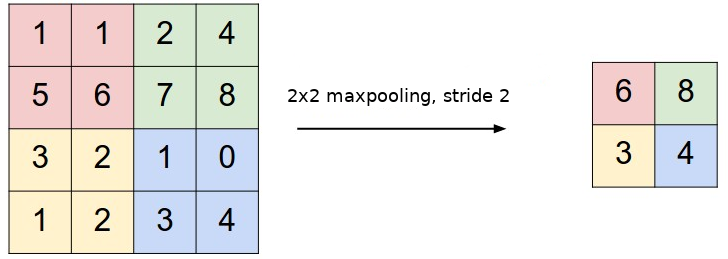
\includegraphics[scale=0.7]{maxpool.png}
  	\caption{Maxpooling med $k=2$ och $s=2$ av ett område med dimensioner $4 \times 4$ där resultatet bildar ett område med dimensionerna $2 \times 2$.}
\end{figure}

Liknande konvolutionslagret utan zero-padding blir det nästintillkommande lagrets dimensioner: \cite{cs231n} \cite{convmath} \cite{convarithmetic}
\begin{equation}
W' = \frac{W-k}{s}+1
\end{equation}
\begin{equation}
H' = \frac{H-k}{s}+1
\end{equation}
\begin{equation}
C' = C
\end{equation}
Antal kanaler förblir konstant. \cite{cs231n} \cite{convmath}

Matematiskt beskrivs maxpoollagret genom: \cite{cs231n} \cite{convmath}
\begin{equation}\label{maxpool}
X^{(l+1)}_{r,c',h',w'} = \underset{0 \leq j < k, \ 0 \leq i < k}{\max} X^{(l)}_{r,c',(h's+j),(w's+i)}
\end{equation}
\subsubsection{Maxpoollagret bakåtpropagering}
Maxpooling saknar vikter och därmed är $\inpd{L(W)}{W^{(l)}}$ tom. Det som återstår är bakåtpropageringen av delta-felet. Med hjälp av kedjeregeln kan man dela upp derivatan i två bråk, $\inpd{L(W)}{X^{(l+1)}_{r,c',h',w'}}$ och $\inpd{X^{(l+1)}_{r,c',h',w'}}{X^{(l)}_{r,c,h,w}}$. $\inpd{L(W)}{X^{(l+1)}_{r,c',h',w'}}$ är den rekursiva delta-delet. $X^{(l+1)}_{r,c',h',w'}$ byts sedan ut mot dess definition enligt ekvation \eqref{maxpool}: \cite{cs231n} \cite{convmath} \cite{webconv3}

\begin{equation}
\begin{split}
	\delta^{(l)}_{r,c,h,w}
		& = \pd{L(W)}{X^{(l)}_{r,c,h,w}} \\
		& = \pd{L(W)}{X^{(l+1)}_{r,c',h',w'}} \pd{X^{(l+1)}_{r,c',h',w'}}{X^{(l)}_{r,c,h,w}} \\
		& = \delta_{r,c',h',w'} \pd{\underset{0 \leq j < k,0 \leq i < k}{\max} X^{(l)}_{r,c',(h's+j),(w's+i)}}{X^{(l)}_{r,c,h,w}} \\
\end{split}
\end{equation}
Den partiella derivatan i den sista ekvationen kommer vara lika med 1 om $X^{(l)}_{r,c',(h's+j),(w's+i)} = X^{(l)}_{r,c,h,w}$. I annat fall kommer $X^{(l)}_{r,c,h,w}$ inte ha någon påverkan på neuron index ${(r,c,h,w)}$ i lager $l+1$ och den partiella derivatan blir lika med 0: \cite{cs231n} \cite{convmath} \cite{webconv3}
\begin{equation}
\delta^{(l)}_{r,c,h,w} = \begin{cases}
				\delta_{r,c,h',w'} & \mbox{om } \begin{split} h = h's+j, \\w = w's+i \end{split}\\
				0 & \mbox{i annat fall}\\
			\end{cases}
\end{equation}

Alltså omdiregeras delta-felet till det ansvariga neuronet vars index kommer att behöva hållas i minnet. Om det finns två eller fler sektioner med samma neuron som är ansvarig för framåtpropageringen så kommer delta-felen summeras från samtliga korresponderande sektioners delta-fel. \cite{cs231n} \cite{convmath} \cite{webconv3}

\subsubsection{Batch Normalization framåtpropagering}
Utan Batch Normalization (BN) är det svårt att få djupa nätverk att konvergera. Detta är till följd av att en liten ändring till det första lagret kan leda till en kaskad av förändringar i de senare lagren. I litteraturen kallas detta för \textit{internal covariate shift}. BN försöker att minimera denna \textit{internal covariate shift} genom att med avseende på alla exempel i mini-hopen normalisera varje \textit{feature map} till varje lager. Resultatet är snabbare konvergens och att det tillåter större träningshastigheter. Följaktligenhar bearbetningen av flera exemepl i taget i en mini-hop en annan praktiska tillämpning än att enbart beräkna konvolutionerna mer tidseffektivt. \cite{cs231n} \cite{batchnorm}

Igen är aktiveringen vid lager $l$ och $l+1$ $X^{(l)} \in \mathbb{R}^{R \times C \times H \times W}$ respektive $X^{(l+1)} \in \mathbb{R}^{R \times C' \times H' \times W'}$. BN har ingen påverkan på dimensionerna av aktiveringen. \cite{cs231n} \cite{batchnorm}

Först beräknas medelvärdena $\mu_c$ och varianserna $\sigma^2_c$ till varje \textit{feature map} $c$: \cite{cs231n} \cite{batchnorm}
\begin{equation}
\mu_c = \frac{1}{RHW} \sum^{R-1}_{r=0} \sum^{H-1}_{h=0} \sum^{W-1}_{w=0} X^{(l)}_{r,c,h,w}
\end{equation}
\begin{equation}
\sigma^2_c  = \frac{1}{RHW} \sum^{R-1}_{r=0} \sum^{H-1}_{h=0} \sum^{W-1}_{w=0} ({X^{(l)}_{r,c,h,w} - \mu_c})^2
\end{equation}
Sedan beräknas den normaliserade aktiveringen $\hat{X}$. Epsilon används för numerisk stabilitet. \cite{cs231n} \cite{batchnorm}
\begin{equation}
\hat{X}_{r,c,h,w} = (X^{(l)}_{r,c,h,w} - \mu_c){(\sigma^2_c)}^{-\frac{1}{2}}
\end{equation}
Sist introduceras 2 vikter, $\gamma_{c'}^{(l)}$ och $\beta_{c'}^{(l)}$, vilka tillåter nätverket att upphäva normaliseringen om nätverket dömmer det att vara användbart. \cite{cs231n} \cite{batchnorm}
\begin{equation}
X^{(l+1)}_{r,c,h,w} = \gamma_{c}^{(l)} \hat{X}_{r,c,h,w} + \beta_{c}^{(l)}
\end{equation}

När nätverket ska köras utanför träning, också kallat \textit{runtime} är det dock inte alltid möjligt att beräkna medelvärdet och variansen av mini-hopen på grund av att man oftast enbart vill testa ett exempel i taget. Medelvärdet och variansen för hela populationen måste då räknas ut och användas i stället för de beräknade värdena. Detta kan göras för små databaser, men om man arbetar med data som innehåller miljontals exempel är det enklare att uppskatta populationens statistik med hjälp av att updatera ett exponensiellt glidande medelvärde (EWMA) vid varje framåtpropagering: \cite{cs231n} \cite{batchnorm}
\begin{equation}
\mu_{EWMA_c} \to \lambda \mu_c + (1-\lambda)\mu_{EWMA_c}
\end{equation}
\begin{equation}
\sigma^2_{EWMA_c} \to \lambda \sigma^2_c + (1-\lambda)\sigma^2_{EWMA_c}
\end{equation}

Där $\mu_{EWMA_c}$ och $\sigma^2_{EWMA_c}$ betecknar de exponensiella glidande medelvärdena och $\lambda$ betecknar dämpfaktorn.


\subsubsection{Batch Normalization bakåtpropagering}
För BN behöver det rekursiva delta-felet $\delta^{(l)}$, derivatan av kostandsfunktionen med avseende på $\gamma_{c'}^{(l)}$ och derivatan av kostandsfunktionen med avseende på $\beta{c'}^{(l)}$ beräknas. För att beräkna detta krävs något som heter kronecker-deltat, oftast betecknat med $\delta_{i,j}$ men kommer vara betecknat med $I_{i,j}$ i denna rapport på grund av $\delta$ används för en annan term. Kronecker-deltat har följande egenskaper: \cite{webBN1} \cite{webBN2}
\begin{equation}\label{kroneckerdelta}
I_{i,j} = \begin{cases} 1 & \mbox{om } i = j \\ 0 & \mbox{om } i \neq j  \end{cases}
\end{equation}
\begin{equation}\label{kroneckerdeltaDERIVATIVE}
\pd{a_{j}}{a_i} = I_{i,j}
\end{equation}
\begin{equation}\label{kroneckerdeltaSUM}
\sum_j  a_i  I_{i,j} = a_j
\end{equation}
Först bryts $\inpd{L(W)}{X^{(l)}}$ upp i tre bråk och sedan summeras alla partiella derivator likt ekvation \eqref{konvolutionbackprop}. \cite{webBN1} \cite{webBN2} Här summeras dessutom R-dimensionen på grund av att aktiveringar från hela mini-hopen har en påverkan på $\delta^{(l)}$.
\begin{align}\label{BN_delta_error}
\begin{split}
	\delta^{(l)}_{r,c,h,w}
		& = \pd{L(W)}{X^{(l)}_{r,c,h,w}} \\
		& = \sum^{R'-1}_{r'=0} \sum^{C'-1}_{c'=0} \sum^{H'-1}_{h'=0} \sum^{W'-1}_{w'=0} \pd{L(W)}{X^{(l+1)}_{r',c',h',w'}} \pd{X^{(l+1)}_{r',c',h',w'}}{\hat{X}_{r',c',h',w'}} \pd{\hat{X}_{r',c',h',w'}}{{X}^{(l)}_{r,c,h,w}}\\
\end{split}
\end{align}

$\inpd{L(W)}{X^{(l+1)}_{r,c,h,w}}$ är det föregående rekursiva delta-felet. $\inpd{X^{(l+1)}_{r',c',h',w'}}{\hat{X}_{r',c',h',w'}}$ hittas enkelt på grund av att den är en linjär funktion. \cite{webBN1} \cite{webBN2}

\begin{equation}\label{BN_dxdxhat}
\begin{split}
	\pd{X^{(l+1)}_{r',c',h',w'}}{\hat{X}_{r',c',h',w'}}
		& = \pd{(\gamma_{c'}^{(l)} \hat{X}_{r',c',h',w'} + \beta_{c'}^{(l)})}{\hat{X}_{r',c',h',w'}} \\
		& =\gamma_{c'}^{(l)}
\end{split}
\end{equation}

För derivatan av den centrerade aktiveringen med avseende på den originella aktiveringen tillämpas produktregeln: \cite{webBN1} \cite{webBN2}
\begin{equation}\label{BN_kedjeregeln}
\begin{split}
\pd{\hat{X}_{r',c',h',w'}}{{X}^{(l)}_{r,c,h,w}} 
	& = \pd{(X^{(l)}_{r',c',h',w'} - \mu_{c'}){(\sigma^2_{c'})}^{-\frac{1}{2}}}{{X}^{(l)}_{r,c,h,w}} \\
	& = {(\sigma^2_{c'})}^{-\frac{1}{2}} \pd{(X^{(l)}_{r',c',h',w'} - \mu_{c'})}{{X}^{(l)}_{r,c,h,w}} - \frac{1}{2}(X^{(l)}_{r',c',h',w'} - \mu_c){(\sigma^2_{c'})}^{-\frac{3}{2}} \pd{\sigma^2_{c'}}{{X}^{(l)}_{r,c,h,w}}
\end{split}
\end{equation}

Derivatan av den första faktorn med avseende på aktiveringen beräknas med hjälp av ekvationer \eqref{kroneckerdelta}, \eqref{kroneckerdeltaDERIVATIVE} och \eqref{kroneckerdeltaSUM}. \cite{webBN1} \cite{webBN2}
\begin{equation}\label{mu'}
\begin{split}
\pd{(X^{(l)}_{r',c',h',w'} - \mu_{c'})}{{X}^{(l)}_{r,c,h,w}}
	& = \pd{({X^{(l)}_{r',c',h',w'} - \frac{1}{RHW} \sum\limits^{R-1}_{r''=0} \sum\limits^{H-1}_{h''=0} \sum\limits^{W-1}_{w''=0} X^{(l)}_{r'',c',h'',w''}})}{{X}^{(l)}_{r,c,h,w}} \\
	& = I_{r',r} I_{c',c} I_{h',h} I_{w',w} - \frac{1}{RHW} I_{c',c}
\end{split}
\end{equation}

Derivatan av den andra faktorn med avseende på aktiveringen beräknas på ett liknande sätt med hjälp av kedjeregeln och ekvationer \eqref{kroneckerdelta}, \eqref{kroneckerdeltaDERIVATIVE} och \eqref{kroneckerdeltaSUM}. \cite{webBN1} \cite{webBN2}
\begin{equation}\label{sigma'}
\begin{split}
\pd{\sigma^2_{c'}}{{X}^{(l)}_{r,c,h,w}}
	& = \pd{\frac{1}{RHW} \sum\limits^{R-1}_{r'=0} \sum\limits^{H-1}_{h'=0} \sum\limits^{W-1}_{w'=0} ({X^{(l)}_{r',c',h',w'} - \mu_{c'}})^2}{{X}^{(l)}_{r,c,h,w}} \\
	& = \frac{1}{RHW} \sum\limits^{R-1}_{r'=0} \sum\limits^{H-1}_{h'=0} \sum\limits^{W-1}_{w'=0} 2 ({X^{(l)}_{r',c',h',w'} - \mu_{c'}}) (I_{r',r} I_{c',c} I_{h',h} I_{w',w} - \frac{1}{RHW} I_{c',c}) \\
	& = \frac{2}{RHW} ({X^{(l)}_{r,c',h,w} - \mu_{c'}})I_{c',c} - \frac{2}{(RHW)^2}  \sum\limits^{R-1}_{r'=0} \sum\limits^{H-1}_{h'=0} \sum\limits^{W-1}_{w'=0} ({X^{(l)}_{r',c,h',w'} - \mu_{c}}) \\
	& = \frac{2}{RHW} ({X^{(l)}_{r,c',h,w} - \mu_{c'}})I_{c',c}
\end{split}
\end{equation}
Den sista summan blir lika med noll på grund av att termerna summeras ihop till medelvärdet minus medelvärdet. 

När alla komponenter till bakåtpropageringen av delta-felet är beräknade är insättning av ekvation \eqref{BN_kedjeregeln}, \eqref{mu'} och \eqref{sigma'} i ekvation \eqref{BN_delta_error} det enda som kvarstår:

\begin{equation}\label{finalBNeq}
\begin{split}
	\delta^{(l)}_{r,c,h,w} 
	& = \sum^{R-1}_{r'=0} \sum^{C'-1}_{c'=0} \sum^{H'-1}_{h'=0} \sum^{W'-1}_{w'=0} \pd{L(W)}{X^{(l+1)}_{r',c',h',w'}} \pd{X^{(l+1)}_{r',c',h',w'}}{\hat{X}_{r',c',h',w'}} \pd{\hat{X}_{r',c',h',w'}}{{X}^{(l)}_{r,c,h,w}}\\
	& = \sum\limits_{r',c',h',w'}\delta^{(l+1)}_{r',c',h',w'} \gamma^{(l)}_{c'} {(\sigma^2_{c'})}^{-\frac{1}{2}} (I_{r',r} I_{c',c} I_{h',h} I_{w',w} - \frac{1}{RHW} I_{c',c}) \\
	& \qquad -\sum\limits_{r',c',h',w'}\delta^{(l+1)}_{r',c',h',w'} \gamma^{(l)}_{c'} \frac{1}{RHW} ({X^{(l)}_{r',c',h',w'} - \mu_{c'}})({X^{(l)}_{r,c',h,w} - \mu_{c'}}) {(\sigma^2_{c'})}^{-\frac{3}{2}} I_{c',c} \\
	& = \delta^{(l+1)}_{r,c,h,w} \gamma^{(l)}_{c} {(\sigma^2_{c})}^{-\frac{1}{2}} - \frac{1}{RHW} \sum\limits_{r',h',w'} \delta^{(l+1)}_{r',c,h',w'} \gamma^{(l)}_{c} {(\sigma^2_{c})}^{-\frac{1}{2}}\\
	& \qquad - \frac{1}{RHW} \sum\limits_{r',h',w'} \delta^{(l+1)}_{r',c,h',w'}\gamma^{(l)}_{c} ({X^{(l)}_{r',c,h',w'} - \mu_{c'}})({X^{(l)}_{r,c,h,w} - \mu_{c}}){(\sigma^2_{c})}^{-\frac{3}{2}} \\
	& = \frac{1}{RHW} \gamma^{(l)}_c {(\sigma^2_{c})}^{-\frac{1}{2}} \biggl(    RHW \delta^{(l+1)}_{r,c,h,w} -  \sum\limits_{r',h',w'} \delta^{(l+1)}_{r',c,h',w'} \qquad \\
	& \qquad -  ({X^{(l)}_{r,c,h,w} - \mu_{c}}) {(\sigma^2_{c})}^{-\frac{3}{2}} \sum\limits_{r',h',w'} \delta^{(l+1)}_{r',c,h',w'} ({X^{(l)}_{r',c,h',w'} - \mu_{c'}}) \biggl) \\
\end{split}
\end{equation}
Derivatan av vikterna hittas på ett liknande sätt som ekvation \eqref{BN_delta_error} till \eqref{finalBNeq}. \cite{webBN1} \cite{webBN2}
\begin{align}
\begin{split}
	\pd{L(W)}{\gamma^{(l)}_{c}}
		& = \sum^{R-1}_{r} \sum^{C'-1}_{c'} \sum^{H'-1}_{h'} \sum^{W'-1}_{w'} \pd{L(W)}{X^{(l+1)}_{r,c',h',w'}} \pd{X^{(l+1)}_{r,c',h',w'}}{\gamma^{(l)}_{c}} \\
		& = \sum^{R-1}_{r} \sum^{C'-1}_{c'} \sum^{H'-1}_{h'} \sum^{W'-1}_{w'} \delta^{(l+1)}_{r,c',h',w'}  \pd{({\gamma_{c'}^{(l)} \hat{X}_{r,c',h',w'} + \beta_{c'}^{(l)}})}{\gamma^{(l)}_{c}} \\
		& = \sum^{R-1}_{r} \sum^{C'-1}_{c'} \sum^{H'-1}_{h'} \sum^{W'-1}_{w'} \delta^{(l+1)}_{r,c',h',w'} \hat{X}_{r,c,h',w'} I_{c',c}\\
		& = \sum^{R-1}_{r} \sum^{H'-1}_{h'} \sum^{W'-1}_{w'} \delta^{(l+1)}_{r,c,h',w'} \hat{X}_{r,c,h',w'} \\
\end{split}
\end{align}


\begin{align}
\begin{split}
	\pd{L(W)}{\beta^{(l)}_{c}}
		& = \sum^{R-1}_{r} \sum^{C'-1}_{c'} \sum^{H'-1}_{h'} \sum^{W'-1}_{w'} \pd{L(W)}{X^{(l+1)}_{r,c',h',w'}} \pd{X^{(l+1)}_{r,c',h',w'}}{\beta^{(l)}_{c}} \\
		& = \sum^{R-1}_{r} \sum^{C'-1}_{c'} \sum^{H'-1}_{h'} \sum^{W'-1}_{w'} \delta^{(l+1)}_{r,c',h',w'}  \pd{({\gamma_{c'}^{(l)} \hat{X}_{r,c',h',w'} + \beta_{c'}^{(l)}})}{\beta^{(l)}_{c}} \\
		& = \sum^{R-1}_{r} \sum^{C'-1}_{c'} \sum^{H'-1}_{h'} \sum^{W'-1}_{w'} \delta^{(l+1)}_{r,c,h',w'} I_{c',c}\\
		& = \sum^{R-1}_{r} \sum^{H'-1}_{h'} \sum^{W'-1}_{w'} \delta^{(l+1)}_{r,c,h',w'} \\
\end{split}
\end{align}

\subsubsection{Softmax framåtpropagering}
Funktionen softmax används i det sista lagret för att gränsa aktiveringen till värden i intervallet $[0,1]$ och har egenskapen att alla prognostiserade värdena i ett exempel från mini-hopen summeras till 1. Om modellen ska klassificiera ett objekt som kan vara av $C$ olika klasser kan $\hat{y}$ tolkas som sannolikheten att objektet är av varje klass $c$; $0 \leq c < C$. \cite{cs231n}

Inmatningsvärde för softmaxlagret är en matris $X^{(l)} \in \mathbb{R}^{R \times C}$ och producerar en matris $X^{(l+1)} \in \mathbb{R}^{R \times C}$ med samma dimensioner. Softmaxlagret definieras enligt:
\begin{equation}
\begin{split}
X^{(l+1)}_{r,c}
	& = \dfrac{e^{X^{(l)}_{r,c}}}{\sum^{C-1}_{c'=0}e^{X^{(l)}_{r,c'}}} \\
\end{split}
\end{equation}

\subsubsection{Softmax bakåtpropagering}

Softmaxlagret saknar vikter och endast det rekursiva delta-felet beräknas vid bakåtpropagering. Kvotregeln, kedjeregeln och kronecker-deltat $I$ används för att härleda den partiella derivatan. Likt de andra lagren summeras de partiella derivatorna på grund av att aktiveringen för ett neuron i lager $l+1$ är en funktion av alla neuron i lager $l$: \cite{cs231n} \cite{notesonbackprop} \cite{websoftmax} 
\begin{equation}
\begin{split}
\delta^{(l)}_{r,c}
		& = \pd{L(W)}{X^{(l)}_{r,c}} \\
		& = \sum^{C-1}_{c'=0} \pd{L(W)}{X^{(l+1)}_{r,c'}} \pd{X^{(l+1)}_{r,c'}}{X^{(l)}_{r,c}} \\
		& = \sum^{C-1}_{c'=0} \delta^{(l+1)}_{r,c} \left(  \dfrac{(e^{X^{(l+1)}_{r,c'}})I_{c',c}}{\sum^{C-1}_{c''=0}e^{X^{(l+1)}_{r,c''}}} - \dfrac{(e^{X^{(l+1)}_{r,c'}})(e^{X^{(l+1)}_{r,c}})}{(\sum^{C-1}_{c''=0}e^{X^{(l+1)}_{r,c''}})^2} \right) \\
		& = \sum^{C-1}_{c'=0}  \delta^{(l+1)}_{r,c} X^{(l+1)}_{r,c'}(I_{c',c}-X^{(l+1)}_{r,c}) \\
		& = \delta^{(l+1)}_{r,c} X^{(l+1)}_{r,c} \left( 1-\sum^{C-1}_{c'=0} X^{(l+1)}_{r,c'} \right)
\end{split}
\end{equation}

\subsection{Praktiska Tillämpningar}
All kod till de exempel på praktiska tillämpningar kan hittas på github: \url{https://github.com/nikitazozoulenko}
\subsubsection{Klassificering av handskrivna siffror}
En enkel CNN-modell kan användas för att klassificera handskriva siffror. För att uppnå detta har MNISTdatabasen för handskriva siffror används. Den består av 60 000 unika exempel av handskrivna siffror. \cite{MNIST}

Låt modellens prognos betecknas med $\hat{y}$. Aktiveringsfunktionen softmax används i det sista lagret för att gränsa värdena till intervallet $[0,1]$ och har egenskapen att alla prognostiserade värdena i ett exempel summeras till 1. Följaktligen kan varje värde i $\hat{y}$ tolkas som sannolikheten att bilden är av varje klass. \cite{cs231n}

\begin{figure}[h]\label{figMNIST}
	\centering
  		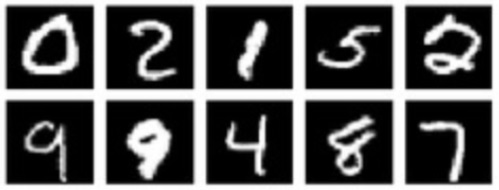
\includegraphics[scale=1]{mnist.png}
  	\caption{Tio bilder av handskrivna siffror från MNISTdatabasen. \cite{MNIST}}
\end{figure}

Input för modellen är en $R \times 1 \times 28 \times 28$ tensor där R står för mini-hopstorleken. Modellen prognostiserar tio värden per bild i form av en tensor $\hat{y} \in \mathbb{R}^{R \times C}$, ett värde för varje klass $C=10$ av siffra. Konstandsfunktionen som har minimerats under träningstiden är funktionen \textit{cross-entropy} betecknat med L. Den verkar på två sannolikhetsfördelningar: De verkliga sannolikheterna $y$ och de prognostiserade sannolikheterna $\hat{y}$: \cite{cs231n} \cite{notesonbackprop}
\begin{equation}
L(W) = - \sum^{R-1}_{r=0} \sum^{C-1}_{c=0}y_{r,c} \ \log{\hat{y}_{r,c}}
\end{equation}
\begin{equation}
\pd{L(W)}{\hat{y}_{r',c'}} = - \frac{y_{r',c'}}{\hat{y}_{r',c'}}
\end{equation}
Endast en modell tränades på grund av begränsningar i datakraft. Den bestod av tre stycken konvolutionsblock, följt med ett softmaxlager (se figur 10). En mini-hopstorlek av 50 användes och 5000 iterationer av framåt- och bakåtpropagering kördes på min egenimplementerade modell skriven i python. Totalt tog det 4 timmar att träna nätverket på min CPU. 

Den slutgiltiga precisionen blev $99.2\%$ på 10 000 nya handskrivna siffror modellen aldrig hade sett tidigare. Av 10 000 handskrivna siffror lyckades modellen klassifisera 9 919 siffror rätt.

\begin{figure}[h]\label{MNISTmodel}
	\centering
  		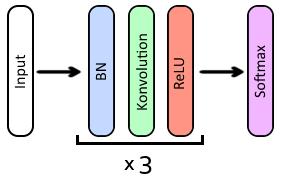
\includegraphics[scale=1.2]{MNISTmodel.png}
  	\caption{Modellen som användes för att läsa av handskrivna siffror. Batch Normalization benämns med BN, konvolution menas en konvolution med kärnstorlek k = 5 och stride s = 2. ReLU är aktiveringsfunktionen Rectified Linear Units och softmax är softmaxlagret.}
\end{figure}

\subsubsection{Ansiktsigenkänning}
Ett konvolutionellt neuralt nätverk är anpassat för att detektera upp till flera tusen ansikten åt gången för realtidsvideo. Modellen producerar ett bestämt antal \textit{boudning boxes}: koordinater som ska detektera alla olika objekt i bilden. Jag utgick från architekturen från RetinaNet från \textit{Focal Loss for Dense Object Detection} (Lin et al.) och anpassade den till $K = 1$ klasser. I varje position i outputlagret föreslår modellen en \textit{boudning box} med fyra koordinater: två punkter för det övre vänstra hörnet respektive nedre hörna hörnet av den positionens \textit{bounding box}. Utöver det förutsägs det $K+1$ sannolikheter att \textit{bounding boxen} innehåller ett objekt av alla $K$ förgrundklasser och 1 bakgrundklass (lådan innehåller inga objekt).\cite{cs231n}\cite{retinanet}

Modellen för objektdetektering går ut på att man utgår från ett antal så kallade anchor boxes vid varje rumslig position i det sista konvolutionella lagret. Om lagret har bredden och höjden $W$ respektive $H$ och $A$ olika storlekar på anchor boxes har lagret totalt $WHA$ olika anchor boxes. Vid träning tilldelas en anchor box ett objekt om dens \textit{intersection over union} (IoU) med den verkliga bounding boxen är större än 0.5 (se figur 11 IoU används för att beräkna hur lika två olika mängder är. I detta fall är mängderna areorna av en anchor box och ett objekts verkliga bounding box. IoU definieras som storleken av snittet av två mänger $A$ och $B$ dividerat med storleken av unionen av $A$ och $B$: \cite{cs231n} \cite{iou}

\begin{equation}
IoU(A, B)=\frac{|A \cap B|}{|A \cup B|}
\end{equation}

\begin{figure}[h]\label{figiou}
	\centering
  		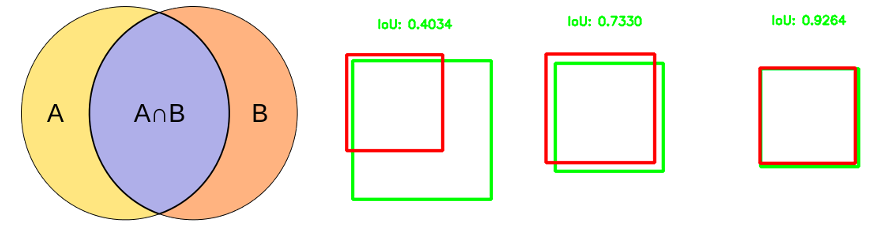
\includegraphics[scale=0.5]{iou.png}
  	\caption{IoU definieras som storleken av snittet av två mänger A och B dividerat med storleken av unionen av A och B. En större IoU medför att prognosen är närmare sanningen. \cite{iou}}
\end{figure}

RetinaNet använder sig av en \textit{feature pyramid}-arkitektur beskriven i \textit{"Feature Pyramid Networks for Object Detection"} (Lin et al.) och en ResNet101 (He et al.) som \textit{backbone}. Featurepyramiden används för att få ut \textit{feature maps} från olika delar av det konvolutionella neurala nätverket för att kunna detektera objekt av olika storlekar. Varje pyramidnivå matas in i ett klassifikationshuvud respektive regressionshuvud (se figur 12) för att räkna ut sannolikheterna att varje anchor box innehåller de $K+1$ olika klasserna, samt att förfina varje anchor box koordinater genom att prognostisera 4 olika offsets för varje sida av anchor boxens bounding box. \cite{resnet} \cite{retinanet} \cite{fpn} 

\begin{figure}[h]\label{figiou}
	\centering
  		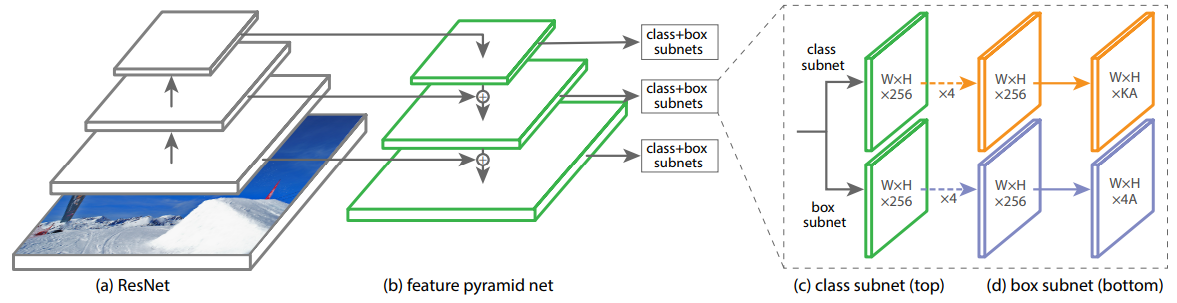
\includegraphics[scale=0.38]{retinanet.png}
  	\caption{RetinaNets arkitektur från \textit{Focal Loss for Dense Object Detection} (Lin et al.). Varje pyramidnivå matas in i ett klassifikationshuvud och ett regressionshuvud. \cite{retinanet}}
\end{figure}

Till skillnad från RetinaNet har min modell, FaceNet, ett mindre antal pyramidnivåer för att lätta på beräkningskraften och för att detektera mindre objekt. RetinaNets anchors har areor från $32^2$ till $512^2$ pixlar spridda över pyramidnivåer P3 till P7. FaceNet använder sig av areor $14^2$ till $220^2$ pixlar spridda över pyramidnivåer P3 till P6. Regressionshuvudet och klassifikations- huvudet i RetinaNet består av 5 konvolutionslager med kärnstorlek 3. Facenet använder istället 2 och 3 konvolutionslager för regressionshuvudet respektive klassifikationshuvudet. I det originala Feature Pyramidnätverket användes linjär interpolation för att göra storleken av högre feature maps större. I FaceNet används k-nearest neighbors (k-NN) istället. ResNet50 användes istället för ett ResNet101 som backbone för att lätta på beräkningskostnaderna. \cite{resnet} \cite{retinanet} \cite{fpn} 

Kostnadsfunktionen som användes var en kombination av Focal Loss (Lin et al.) och Smooth L1 Loss. FaceNet använder samma hyperparametrar som uppnådde bästa resultat för RetinaNet: $\alpha = 3$ för förgrundklassen och $\gamma=2$. \cite{retinanet}

\begin{equation}
L_r(x) = \begin{cases}
				0.5x^2 & \mbox{om } |x| < 1\\
				|x| - 0.5 & \mbox{i annat fall}\\
			\end{cases}
\end{equation}

\begin{equation}
L_c(p, \hat{p}) = - \alpha (1-p)^{\gamma}p \log{\hat{p}}
\end{equation}

\begin{equation}
\begin{split}
	L(W) = & \sum_{k \in pyramid} \frac{1}{N^k_c} \sum_{a \in anchors} L_r(r_a - \hat{r}_a) \\ 
	& + \sum_{k \in pyramid} \frac{1}{N^r_c} \sum_{a \in anchors} L_c(p_a, \hat{p}_a)  \\ 
\end{split}
\end{equation}

$N^k_c $ och $N^k_r $ betäcknar alla anchors som deltar i klassifikationskonstnaden respektive regressionskonstnaden i pyramidnivå $k$. För klassifikationskonstnaden är $\hat{p}$ 1 för alla anchors som har blivit tillgivna ett objekt och 0 för alla som bara innehåller bakgrundsklassen. Endast anchors som innehåller ett objekt deltar i regressionskostnaden. $r_a$ innehåller de 4 koordinaterna den slutgiltiga boudning boxen har.

Modellen tränades i 350 000 iterationer med en mini-hopsstorlek av 3. Träningshastigheten började på 0.005 och dividerades med 10 vid 200 000 iterationer. Varje träningsexempels storlek gjordes slumpmässigt om till $512^2$, $576^2$ eller $640^2$ pixlar och speglades horizontellt med sannolikhet 0,5 för att artificiellt utöka mängden träningsdata. Den totala träningstiden var 18 timmar på en NVIDIA GTX 1080ti. Figur 13 visar kvantitativa resultat från WIDERFace valideringsdata.

En iteration av framåtpropageringen tar 20 ms vilket möjliggör att modellen kan köras i realtid, 50 gånger i sekunden.

\begin{figure}[h]\label{results1}
	\centering
  		
\includegraphics[scale=0.42]{results1.png}
  	\caption{Kvantitativa resultat från valideringsdatan från WIDERFace: Bilder som modellen aldrig har sett tidigare.}
\end{figure}

\section{Diskussion}
Den matematiska modellen av artificiella neurala nätverk och konvolutionella neurala nätverk, samt bakåt- och framåtpropagering förklaras och härleds i sektion 3.2 och 3.3. Ett exempel på hur modellen kan tillämpas är att klassificera handskrivna siffror, som i sektion 3.4.1. 
En annan möjlighet är att anpassa ett konvolutionellt neuralt nätverk för att detektera alla ansikten i en digital bild. På grund av att en iteration av algoritmen tar 20 ms är det möjligt att köra modellen i realtid. Det kan exempelvis användas i övervakningskameror eller inom robotik för att känna igen människoansikten i realtid. 

Algoritmen är dock inte perfekt och har flera brister. Modellen prognostiserar att det finns ansikten på flera ställen där det inte finns några i verkligheten. För att undankomma detta låter jag endast modellen visa upp bounding boxes med sannolikhet större än 0.5 att det finns ett ansikte där. Resultatet blir att modellen inte hittar 100\% av all ansikten i bilden (se figur 13). Ytterligare har modellen problem med små ansikten. Detta är dels på grund av att modellen inte kan urskilja ett ansikte med så lite information (ca minimum $10^2$ pixlar per ansikte), och dels för att FaceNet prognostiserar ca 30 000 olika anchors för de minsta storlekarna. Detta leder till att klassifikationskostnaden består av till mestadels negativa exempel. Delta-felet av bakgrundsklasserna dominerar och gör att delta-felet av förgrundsklassen (ansikten) inte har en stor påverkan på den slutgiltiga gradienten.

\section{Källkritik}
\subsection{CS231n: Convolutional Neural Networks for Visual Recognition}
Angående äkthetskriteriet är källan en kurs utgiven av Stanford, ett av världens mest prestigefulla universitet. Kursen är gjord av Fei-Fei Li och Andrej Karpathy vilka är experter inom området Deep learning. Fei-Fei Li har varit författare för över 100 olika publicerade vetenskapliga artiklar inom maskininlärning och är professor på Stanford. Andrej Karpathy är en doktorand från Stanford och har arbetet för bland annat Google, DeepMind och OpenAI. Just nu arbetar han som "Director of AI" hos Tesla. Informationen i kursen kommer från experter inom området.

Enligt tendenskriteriet är källan opartisk. Stanford är en av de mest prestigefulla universiteten i världen och skulle inte riskera att ge ut felaktig eller vinklad information. Det skulle dessutom försämra föreläsarnas rykten inom forskarvärlden.

Angående beroendekriteriet är källan en kombination av att vara en förstahandskälla och andrahandskälla. Å ena sidan kan Li och Karpathy bidra med deras egen forskning som en förstahandskälla, men å andra sidan är majoriteten av undervisningsmaterialet inte något som förelasarna själv har kommit på.

Enligt tidskriteriet ligger källan bra till. Kursen är endast två år gammal och innehåller den nyaste tekniken inom deep learning. Trots att maskininlärning är ett snabbt växande område spelar det inte en stor roll att kursen är två år gammal för att kursen lär ut grunderna inom konvolutionella neurala nätverk för dataseende: De nya upptäckterna som sker efter kursen gavs ut är inte relevanta för målgruppen.

\subsection{Batch normalization: Accelerating deep network training by reducing internal covariate shift.}
Källan är en vetenskaplig artikel av Sergey Ioffe och Christian Szegedy. De är båda doktorander och forskare på Google. Deras forsking och denna källa har varit kritisk för den fortsatta utvecklingen för neurala nätverk och deep learning. Enligt äkthetskriteriet är källan trovärdig. Pappret har genomgått peer review och har implementerats hundratals gånger av olika företag och privatpersoner i flera olika modeller. Detsamma gäller tendenskriteriet.

Enligt beroendekriteriet är källan en förstahandskälla. Källan beskriver forskningen som Ioffe och Szegedy har genomfört. 

Angående tidskriteriet är källan av hög kvalité. Den vetenskapliga artikeln var publicerad år 2015 och innehåller moderna tekniska framsteg inom deep learning. Källan är digitaliserad och har ingen risk att bli utsatt för narrativ smitta på grund av att originalpappret är spriden och arkiverad över nätet. 

\begin{thebibliography}{99}	
\bibitem{cs231n} 
	\textit{CS231n: Convolutional Neural Networks for Visual Recognition.}
    F. Li, A. Karpathy och J. Johnson.
	Stanford University, föreläsning, vinter 2016.
	
\bibitem{notesonbackprop} 
	\textit{Notes on Backpropagation.}
    P. Sadowski.
    University of California Irvine	Department of Computer Science.
    
\bibitem{convmath} 
	\textit{Introduction to Convolutional Neural Networks.}
    J. Wu. 
    National Key Lab for Novel Software Technology, Nanjing University, Kina.
    1 maj, 2017.

\bibitem{convarithmetic} 
	\textit{A guide to convolution arithmetic for deep learning.}
    V. Dumoulin  och F. Visin.
    FMILA, Université de Montréal. AIRLab, Politecnico di Milano.
	24 mars, 2016.

\bibitem{highperformanceconv} 
	\textit{High Performance Convolutional Neural Networks for Document Processing.}
    K. Chellapilla, S. Puri, P. Simard.
    Tenth International Workshop on Frontiers in Handwriting Recognition. 
    La Baule, Frankrike, Suvisoft.
	Oktober 2006.

\bibitem{wikiStanford} 
	\textit{Unsupervised Feature Learning and Deep Learning.}
    Standford University, Department of Computer Science.
    URL http://ufldl.stanford.edu/wiki/.
	Senast uppdaterad 31 mars 2013.
	
\bibitem{gradient} 
	\textit{Scientific Computing 2013, Worksheet 6: Optimization: Gradient and steepest descent.}
    University of Tartu, Estland.
    2013.
    
\bibitem{yolo} 
	\textit{You only look once: Unified, real-time object detection.}
    J. Redmon, S. Divvala, R. Girshick, och A. Farhadi. 
    arXiv preprint arXiv:1506.02640, 2015.
    
\bibitem{batchnorm} 
	\textit{Batch normalization: Accelerating deep network training by reducing internal covariate shift.}
    S. Ioffe och C. Szegedy. 
	arXiv preprint arXiv:1502.03167, 2015.
    
\bibitem{webconv1} 
	\textit{Backpropagation In Convolutional Neural Networks.}
	J. Kafunah.
    DeepGrid, Organic Deep Learning. 
    URL http://www.jefkine.com/.
	5 september 2016.

\bibitem{webBN1} 
	\textit{What does the gradient flowing through batch normalization looks like?}
	C. Thorey.
    Machine Learning Blog. 
    URL http://cthorey.github.io/.
	28 januari 2016.
	
\bibitem{webconv2} 
	\textit{Note on the implementation of a convolutional neural networks.}
	C. Thorey.
    Machine Learning Blog. 
    URL http://cthorey.github.io/.
	2 februari 2016.
	
\bibitem{webBN2} 
	\textit{Understanding the backward pass through Batch Normalization Layer.}
	Flaire of Machine Learning
    URL https://kratzert.github.io.
	5 september 2016.
	
\bibitem{webconv3} 
	\textit{Convolutional Neural Networks.}
	A. Gibiansky.
    URL http://andrew.gibiansky.com.
	24 februari 2014.
	
\bibitem{websoftmax} 
	\textit{Classification and Loss Evaluation - Softmax and Cross Entropy Loss.}
	P. Dahal. 
	DeepNotes.
    URL https://deepnotes.io/softmax-crossentropy.
	24 februari 2014.
	
\bibitem{MNIST}
	\textit{The MNIST database of handwritten digits}
	Y. LeCun, C. Cortes och C. Burges. Courant Institute, NYU. Google Labs, New York. Microsoft Research, Redmond. 
	URL http://yann.lecun.com/exdb/mnist/.
	Hämtad 3 november 2017.
	
\bibitem{figSGD}
	\textit{Pygradsc.}
	J. Komoroske.
	URL https://github.com/joshdk/pygradesc.
	12 oktober 2012.
	
\bibitem{figboatcnn}
	\textit{Understanding Convolutional Neural Networks for NLP.}
	D. Britz.
	WildML, Artificial Intelligence, Deep Learning, and NLP.
	7 november 2015.
	
\bibitem{figkonv}
	\textit{Understanding Convolutional Neural Networks for NLP.}
	D. Britz.
	WildML, Artificial Intelligence, Deep Learning, and NLP.
	7 november 2015.
	
\bibitem{figconv}
	\textit{Deep learning for complete beginners: convolutional neural networks with keras.}
	P. Veličković.
	Camebridge Spark. 
	URL https://cambridgespark.com/content.
	Senast uppdaterad 20 mars 2017.


\bibitem{resnet} 
	\textit{Deep residual learning for image recognition.}
    K. He, X. Zhang, S. Ren, och J. Sun. 
    arXiv preprint arXiv:1512.03385, 2015.

\bibitem{iou}
	Jaccard Index. Wikipedia.
    URL https://en.wikipedia.org/wiki/Jaccard{\_}index. 
    Hämtad 20 januari 2018
    
\bibitem{retinanet}
	\textit{Focal Loss for Dense Object Detection.}
	Tsung{-}Yi Lin,
    Priya Goyal,
    Ross B. Girshick,
    Kaiming He and
    Piotr Doll{\'{a}}r.
    arXiv preprint arXiv:1708.02002, 2017

\bibitem{fpn}
	\textit{Feature Pyramid Networks for Object Detection.}
	Tsung{-}Yi Lin,
               Piotr Doll{\'{a}}r,
               Ross B. Girshick,
               Kaiming He,
               Bharath Hariharan and
               Serge J. Belongie.
    arXiv preprint arXiv:1612.03144, 2016
    
\bibitem{WIDERFace}
	\textit{WIDER FACE: A Face Detection Benchmark.}
	Yang, Shuo and Luo, Ping and Loy, Chen Change and Tang, Xiaoou
    IEEE Conference on Computer Vision and Pattern Recognition (CVPR), 2016

\end{thebibliography}


\end{document}